% Created 2018-06-03 Sun 07:51
% Intended LaTeX compiler: pdflatex
% Template: Diogo Ferrari
\documentclass[a4paper]{article}
% === Packages =================================
\usepackage{./sty/basic-article}
\usepackage{./sty/math-commands}
\usepackage{./sty/math-commands-thm}
% === Document =================================
                  % ================================================
% ================================================
\author{Diogo Ferrari}
\date{\textit{[2018-05-25 Fri 14:01]}}
\title{Exploratory Data Analysis in R (edar)}
\hypersetup{
 pdfauthor={Diogo Ferrari},
 pdftitle={Exploratory Data Analysis in R (edar)},
 pdfkeywords={},
 pdfsubject={},
 pdfcreator={Emacs 25.2.2 (Org mode 9.1.13)}, 
 pdflang={English}}
\begin{document}

\maketitle
\tableofcontents


\section{Introduction}
\label{sec:org7e8f689}

The package Exploratory Data Analysis in R (edar) allows efficient exploratory data analyses with few lines of code. It contains some functions to:
\begin{itemize}
\item overview and summarise the data set
\item check balance of covariates among control and treatment groups
\item create organized and ready to export (to latex, html, etc) tables with results of model estimation
\item easily create plots with fitted values comparing one or more models under different treatment conditions
\item create plots with point estimates and their intervals (dotwisker plots)
\item conduct robustness checks of the model results (multiple imputation, post-stratification, etc). 

Quantitative researchers conduct those tasks repeatedly. The package provides functions to do them more efficiency and with minimum code.
\end{itemize}


\begin{enumerate}
\item Check the numerical and categorical variables of the data set
\begin{itemize}
\item Look for outliers and missing values
\item Check distribution of the variables
\end{itemize}
\item \label{org23ca5ec} Fit a multivariate regression model
\item \label{orgf389d1d} Display and check the results
\item Do multiple imputation and post-stratification (in surveys)
\item Repeat \ref{org23ca5ec} and \ref{orgf389d1d}
\item \label{orgfcfa6c3} Recode some Variables or change model specifications
\item Repeat
\end{enumerate}

Execpt for item \ref{orgfcfa6c3}, the package \texttt{edar} can spead up all those tasks. For instance, suppose \texttt{data} contains the data set. Those tasks can be performed with few lines of code:

\lstset{numbers=left,language=r,label= ,caption= ,captionpos=b}
\begin{lstlisting}
# summary tables
data %>% summarise_alln(.) # summarise all numerical variables of the data in a table
data %>% summarise_allc(.) # summarise all categorical variables of the data in a table 
data %>% summarise_allcbundle(.) # summarise all categorical variables of the data in a table
data %>% ebalance(., treatmentVar="treat") ## summary of numerical variables for different levels of "treat"

# summary plots
data %>% gge_describe(.)  ## marginal distribution of all variables
data %>% gge_density(.) ## marginal distribution of numerical variables only
data %>% gge_histogram(.)## marginal distribution of numerical variables only using histograms
data %>% gge_barplot(.) ## marginal distribution of non-numerical variables

# afeter fitting the models model1, model2, etc ...
tidye(model1, hc=T) ## summarise put summary in a tidy data.frame (using robust std.errors)
tidye(list(model1,model2)) ## same, but summarise both models at once

# plots
gge_coef(model1) ## dotwisker plot (plot with coefficients and std. errors)
model %>%  gge_fit(., data, "y", "x1") ## plot with fitted values as function of covariate x1

# multiple imputation and post-stratification
emultimputation(data, formula,  dep.vars = c(...), ind.vars=c(...)) 
epoststrat(data, population.proportion, strata = ~ stratification.variable1 + stratification.variable2...) 
\end{lstlisting}

\section{Workflow}
\label{sec:org5478a81}
\subsection{Data}
\label{sec:org941c5e3}
Here is an example of workflow with \texttt{edar}. We will use the data set \texttt{edar\_survey} that comes with the package:

\lstset{numbers=left,language=r,label=orgb6b50b5,caption= ,captionpos=b}
\begin{lstlisting}
library(magrittr)
library(edar)

data(edar_survey)
help(edar_survey)

data = edar_survey
\end{lstlisting}

\lstset{numbers=left,language=ascii,label=orgce69283,caption= ,captionpos=b}
\begin{lstlisting}
A National Survey from Brazil
Description:

     The data set is a subset of a national suvery conducted in Brazil
     in 2013. The survey measures preferences of individuals for
     interpersonal and interregional redistribution of income as well
     as preferences for centralization of political authority.

Usage:

     data(edar_survey)
     
Format:

     A data frame with 700 rows and 16 columns:

     gender factor with "men" and "woman"

     educ factor with "high" if the individual completed high school or
          more, and "low" otherwise

     age integer with age in years

     yi numeric variable with household income per capita

     yi.iht inverse hyperbolic transformation of yi

     state factor with the state in which the individual lives

     region factor with macroregion

     ys.mean average household percapita income in the state, computed
          using the 2013 Brazilian National Household Survey (PNAD)

     trust factor, "high" or "low" trust in the federal government

     treat numeric, 0 for control group or 1 for treatment group. It is
          a randomly generated variable for used for ilustration of the
          examples and vignettes only

     ys.gini numeric, Gini coefficient of the state computed using the
          2013 Brazilian National Household Survey (PNAD)

     racial.frag.ratio numeric, racial fractionalization at the state
          over racial fractionalization at the national level

     reduce.income.gap factor, "A"=Agree, "A+"=Strongly Agree,
          "D"=Disagree, "D+"=Strongly Disagree, "N"=Neither Agree or
          Disagree that "Government should reduce income gap between
          rich and poor"

     transfer.state.tax factor, "A"=Agree, "A+"=Strongly Agree,
          "D"=Disagree, "D+"=Strongly Disagree, "N"=Neither Agree or
          Disagree that the "Government should redistribute resources
          from rich to poor states"

     minimum.wage factor, captures the answer to "Who should decide
          about the minimum wage policy?". The levels are "Each city
          should decide", "Each state should decide", "Should be the
          same accros the country"

     unemployment.policy factor, captures the answer to "Who should
          decide about the unemployment policy?". The levels are "Each
          city should decide", "Each state should decide", "Should be
          the same accros the country"

     red.to.poor factor, captures the answer to "Who should decide
          about policies to redistribute income to poor?". The levels
          are "Each city should decide", "Each state should decide",
          "Should be the same accros the country"

Source:

     <URL: http://web.fflch.usp.br/centrodametropole/>
\end{lstlisting}


\subsection{Summary tables}
\label{sec:org9b09e67}
First, we can have a quick overview of the data set using the functions \texttt{summarise\_alln} and \texttt{summarise\_allc} provided by \texttt{edar} package. They show the summary of numerical and categorical variables in the data set, respectively:

NOTE: throughout this document, I use the package \texttt{kable} for better visualization of some tables

\lstset{numbers=left,language=r,label= ,caption= ,captionpos=b}
\begin{lstlisting}
data %>% 
    summarise_alln(., digits=2) %>%
    kableExtra::kable(., "latex", booktabs = T ) %>%
    kableExtra::kable_styling(latex_options = c("scale_down"))
\end{lstlisting}

\begin{table}[H]
\centering
\resizebox{\linewidth}{!}{
\begin{tabular}{lrrrrrrrrrrrr}
\toprule
var & N & NAs & Mean & sd & se & Median & Min & Max & q.025 & q.25 & q.75 & q.975\\
\midrule
age & 700 & 0 & 45.35 & 16.43 & 0.62 & 45.00 & 18.00 & 92.00 & 18.00 & 32.00 & 57.00 & 78.52\\
racial.frag.ratio & 700 & 0 & 0.87 & 0.14 & 0.01 & 0.87 & 0.49 & 1.05 & 0.49 & 0.86 & 0.96 & 1.05\\
treat & 700 & 0 & 0.48 & 0.50 & 0.02 & 0.00 & 0.00 & 1.00 & 0.00 & 0.00 & 1.00 & 1.00\\
yi & 618 & 82 & 930.61 & 1544.16 & 62.12 & 600.00 & 0.00 & 20000.00 & 83.93 & 300.00 & 1000.00 & 4985.83\\
yi.iht & 618 & 82 & 6.96 & 1.08 & 0.04 & 7.09 & 0.00 & 10.60 & 5.12 & 6.40 & 7.60 & 9.21\\
\addlinespace
ys.gini & 700 & 0 & 0.53 & 0.03 & 0.00 & 0.52 & 0.43 & 0.59 & 0.49 & 0.51 & 0.54 & 0.59\\
ys.mean & 700 & 0 & 973.50 & 300.26 & 11.35 & 792.04 & 559.83 & 2011.37 & 573.39 & 688.08 & 1233.07 & 1347.29\\
\bottomrule
\end{tabular}}
\end{table}


\lstset{numbers=left,language=r,label= ,caption= ,captionpos=b}
\begin{lstlisting}

data %>% summarise_allc(.) %>% print(width=70)

\end{lstlisting}

\begin{verbatim}
# A tibble: 10 x 7
   var        N   NAs Categories Frequency     Table Categories.Labe…
   <chr>  <dbl> <int>      <int> <chr>         <lis> <chr>           
 1 educ     700     0          2 high  (39.71… <dat… high, low       
 2 gender   700     0          2 man   (41.29… <dat… man, woman      
 3 minim…   695     5          4 Each  (8.63 … <dat… Each city shoul…
 4 red.t…   679    21          4 Each  (11.78… <dat… Each city shoul…
 5 reduc…   700     0          5 A     (72.43… <dat… A, A+, D, D+, N 
 6 region   700     0          5 CO    (6.14 … <dat… CO, NE, NO, SE,…
 7 state    700     0         27 AC    (0.29 … <dat… AC, AL, AM, AP,…
 8 trans…   700     0          5 A     (70.14… <dat… A, A+, D, D+, N 
 9 trust    694     6          3 high  (56.92… <dat… high, low       
10 unemp…   699     1          4 Each  (9.59 … <dat… Each city shoul…
\end{verbatim}


The summary of categorical variables produced by \texttt{summarise\_allc} contains a column named \texttt{Table}, which contains a table with the counts for each category value of the variable.

\lstset{numbers=left,language=r,label=org19b65d4,caption= ,captionpos=b}
\begin{lstlisting}
tab = data %>% summarise_allc(.)
tab$Table[[6]]
\end{lstlisting}

\begin{center}
\begin{tabular}{lrrrrrr}
Variable & CO & NE & NO & SE & SU & NA\\
\hline
region & 43 & 333 & 46 & 174 & 104 & 0\\
\end{tabular}
\end{center}

It is common to have data sets in which many categorical variables have the same categories. The function \texttt{summarise\_allcbundle} provides a summary of all categorical variables of the data set and aggregate those with same categories. The output contain columns named \texttt{Table}, \texttt{Tablep}, and \texttt{Tablel}. \texttt{Table} contains a table with counts of the categories of the variables. \texttt{Tablep} presents the same information, but in percentage. \texttt{Tablel} presents both the counts and percentage, which can be exported directly for reports and articles. The column \texttt{Variables} in the output contains the name of all the variables that have the same \texttt{Category.Labels}

\lstset{numbers=left,language=r,label= ,caption= ,captionpos=b}
\begin{lstlisting}
data %>% summarise_allcbundle(.)  %>% print(., width=70)
\end{lstlisting}

\begin{verbatim}
# A tibble: 6 x 6
  N.Variables Variables Categories.Labels      Table   Tablep  Tablel
        <int> <list>    <chr>                  <list>  <list>  <list>
1           2 <chr [2]> A, A+, D, D+, N        <data.… <data.… <data…
2           1 <chr [1]> AC, AL, AM, AP, BA, C… <data.… <data.… <data…
3           1 <chr [1]> CO, NE, NO, SE, SU     <data.… <data.… <data…
4           3 <chr [3]> Each city should deci… <data.… <data.… <data…
5           2 <chr [2]> high, low              <data.… <data.… <data…
6           1 <chr [1]> man, woman             <data.… <data.… <data…
\end{verbatim}



\lstset{numbers=left,language=r,label= ,caption= ,captionpos=b}
\begin{lstlisting}
tab = data %>% summarise_allcbundle(.)
tab$Table[[5]]
\end{lstlisting}

\begin{center}
\begin{tabular}{lrrr}
Variable & high & low & NA\\
\hline
educ & 278 & 422 & 0\\
trust & 395 & 299 & 6\\
\end{tabular}
\end{center}

\begin{center}
\begin{tabular}{lrrr}
Variable & high & low & NA\\
\hline
educ & 278 & 422 & 0\\
trust & 395 & 299 & 6\\
\end{tabular}
\end{center}



\lstset{numbers=left,language=r,label=org4725b74,caption= ,captionpos=b}
\begin{lstlisting}
tab$Tablep[[5]]
\end{lstlisting}

\begin{center}
\begin{tabular}{lrrr}
Variable & high & low & NA\\
\hline
educ & 39.71 & 60.29 & 0\\
trust & 56.43 & 42.71 & 0.86\\
\end{tabular}
\end{center}



\lstset{numbers=left,language=r,label=orgeac9403,caption= ,captionpos=b}
\begin{lstlisting}
tab$Tablel[[5]]
\end{lstlisting}

\begin{center}
\begin{tabular}{llll}
Variable & high & low & NA\\
\hline
educ & 39.71 \% (N=278) & 60.29 \% (N=422) & 0 \% (N=0)\\
trust & 56.43 \% (N=395) & 42.71 \% (N=299) & 0.86 \% (N=6)\\
\end{tabular}
\end{center}

\subsection{Checking balance of covariates}
\label{sec:org6128e09}

We can easily check the distribution of covariates among two factor levels. Consider the variable \texttt{treat}, which represents the treatment condition (1=treatment, 0=control). We can describe the distribution of covariates using \texttt{ebalance()}. The table follows recomendations in \cite{imbens2015causal}.

\lstset{numbers=left,language=r,label=org341f080,caption= ,captionpos=b}
\begin{lstlisting}
data %>% ebalance(., treatmentVar='treat') %>% print(., digits=2)

\end{lstlisting}

\begin{center}
\begin{tabular}{lrrrrrrrr}
Variable & mut & st & muc & sc & NorDiff & lnRatioSdtDev & pit & pic\\
\hline
age & 45.83 & 16.61 & 44.9 & 16.27 & 0.06 & 0.02 & 0.03 & 0.06\\
yi & 946.36 & 1671.84 & 916.04 & 1418.32 & 0.02 & 0.16 & 0.03 & 0.07\\
yi.iht & 6.95 & 1.07 & 6.98 & 1.08 & -0.03 & -0.01 & 0.03 & 0.07\\
ys.mean & 981.54 & 297.97 & 966.04 & 302.6 & 0.05 & -0.02 & 0.04 & 0.02\\
ys.gini & 0.52 & 0.03 & 0.53 & 0.03 & -0.16 & -0.1 & 0.03 & 0.05\\
racial.frag.ratio & 0.87 & 0.13 & 0.87 & 0.14 & 0.02 & -0.07 & 0 & 0.05\\
MahalanobisDist & nil & nil & nil & nil & 0.22 & nil & nil & nil\\
pscore & 0.5 & 0.5 & 0.46 & 0.5 & 0.07 & 0 & 0.02 & 0.04\\
LinPscore & -0.09 & 26.61 & -1.92 & 26.54 & 0.07 & 0 & 0.04 & 0.07\\
N & 337 & nil & 363 & nil & nil & nil & nil & nil\\
\end{tabular}
\end{center}

\subsection{Summary plots}
\label{sec:org5eb2bec}

The package also provides some functions to easily visualise the marginal distribution of many variables at once. The marginal densities can be grouped by factors using the parameter \texttt{group}. When the marginal densities are presented by group, the plot include the p-value of the Kolmogorov-Smirnov distance.

\lstset{numbers=left,language=r,label= ,caption= ,captionpos=b}
\begin{lstlisting}
g = data[,1:8] %>% gge_describe(.)
print(g)
\end{lstlisting}

\begin{center}
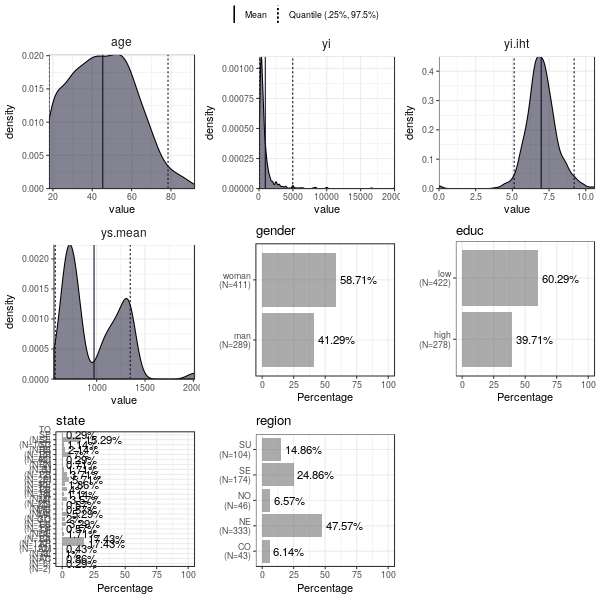
\includegraphics[width=.9\linewidth]{gge_describe.png}
\end{center}



\lstset{numbers=left,language=r,label= ,caption= ,captionpos=b}
\begin{lstlisting}
g = data[,1:9] %>% gge_describe(., group='educ')
print(g)
\end{lstlisting}

\begin{center}
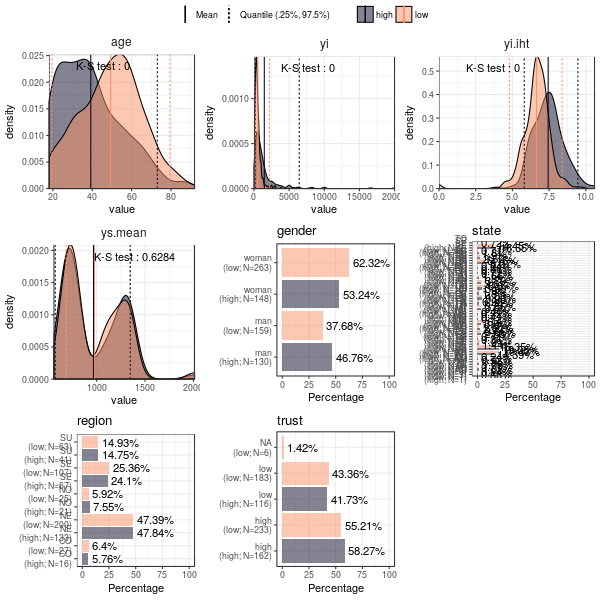
\includegraphics[width=.9\linewidth]{gge_describe_group.png}
\end{center}


Other similar functions provided by the package are:
\begin{itemize}
\item gge\_barplot()
\item gge\_density()
\item gge\_histogram()
\item gge\_barplot()
\end{itemize}
\subsection{Analyzing output of model estimation}
\label{sec:orgc35e977}
\subsubsection{Fitting models}
\label{sec:orgb4ae9c3}

The package \texttt{edar} make it easy to display results of estimation. It can be achieved with minimum code. Suppose we estimated five different models:

\lstset{numbers=left,language=r,label=orgbd24fed,caption= ,captionpos=b}
\begin{lstlisting}
set.seed(77)
data = tibble::data_frame(n = 300,
                          x1   = rnorm(n,3,1),
                          x2   = rexp(n),
                          cat1 = sample(c(0,1), n, replace=T),
                          cat2 = sample(letters[1:4], n, replace=T),
                          y    = -10*x1*cat1 + 10*x2*(3*(cat2=='a') -3*(cat2=='b') +1*(cat2=='c') -1*(cat2=='d')) + 
                              rnorm(n,0,10), 
                          y.bin = ifelse(y < mean(y), 0, 1),
                          y.mul = 1+ifelse( - x1 - x2 + rnorm(n,sd=10) < 0, 0,
                                    ifelse( - 2*x2 + rnorm(n,sd=10) < 0, 1, 2)),
                          )

formula1    = y ~ x1
formula2    = y ~ x1 + x2
formula3    = y ~ x1*cat1 + x2*cat2
formula4bin = y.bin ~ x1+x2*cat2
formula4bin1 = y.bin ~ x1+x2
formula4bin2 = y.bin ~ x1*cat1+x2*cat2
formula5mul = y.mul ~ x1 + x2

model.g1    = lm(formula1, data)
model.g2    = lm(formula2, data)
model.g3    = lm(formula3, data)
model.bin   = glm(formula4bin, data=data, family='binomial')
model.bin1  = glm(formula4bin, data=data, family='binomial')
model.bin2  = glm(formula4bin, data=data, family='binomial')
model.mul   = nnet::multinom(formula5mul, data)

\end{lstlisting}

\subsubsection{Tables}
\label{sec:orgf9d1ad3}
We want to vizualize the model estimate. The function \texttt{tidye} creates tidy summary tables with the output. It is a wrap function for \texttt{broom::tidy()}, and it works with list of models. Here are some examples:

\lstset{numbers=left,language=r,label= ,caption= ,captionpos=b}
\begin{lstlisting}

tidye(model.g3)

## works with other types of dependent variables
# tidye(model.bin)
# tidye(model.mul)

\end{lstlisting}

\begin{center}
\begin{tabular}{lrrrrrr}
term & estimate & std.error & conf.low & conf.high & statistic & p.value\\
\hline
(Intercept) & 3.6042 & 3.0375 & -2.3742 & 9.5826 & 1.1866 & 0.2364\\
x1 & -0.9053 & 0.8167 & -2.5126 & 0.7021 & -1.1085 & 0.2686\\
cat1 & -2.2011 & 3.6151 & -9.3164 & 4.9142 & -0.6089 & 0.5431\\
x2 & 28.0061 & 1.3544 & 25.3403 & 30.6719 & 20.6774 & 0\\
cat2b & -0.1835 & 2.3532 & -4.8151 & 4.4481 & -0.078 & 0.9379\\
cat2c & -0.9414 & 2.2746 & -5.4184 & 3.5355 & -0.4139 & 0.6793\\
cat2d & -1.4556 & 2.4636 & -6.3044 & 3.3932 & -0.5909 & 0.5551\\
x1:cat1 & -9.2755 & 1.1527 & -11.5442 & -7.0069 & -8.0471 & 0\\
x2:cat2b & -58.1667 & 1.8639 & -61.8352 & -54.4982 & -31.2071 & 0\\
x2:cat2c & -17.6127 & 1.7246 & -21.0071 & -14.2183 & -10.2125 & 0\\
x2:cat2d & -38.3783 & 2.0687 & -42.4499 & -34.3068 & -18.5523 & 0\\
\end{tabular}
\end{center}

We can have robust standard errors, and keep or not information of non-corrected values for comparison.

\lstset{numbers=left,language=r,label= ,caption= ,captionpos=b}
\begin{lstlisting}
## with robust std.errors
tidye(model.g3, hc=T)

\end{lstlisting}

\begin{center}
\begin{tabular}{lrrrrrr}
term & estimate & std.error & conf.low & conf.high & statistic & p.value\\
\hline
(Intercept) & 3.6042 & 3.2952 & -2.8544 & 10.0628 & 1.0938 & 0.275\\
x1 & -0.9053 & 0.8481 & -2.5676 & 0.7571 & -1.0673 & 0.2867\\
cat1 & -2.2011 & 3.7761 & -9.6023 & 5.2001 & -0.5829 & 0.5604\\
x2 & 28.0061 & 1.5784 & 24.9124 & 31.0998 & 17.7432 & 0\\
cat2b & -0.1835 & 2.5577 & -5.1965 & 4.8295 & -0.0717 & 0.9429\\
cat2c & -0.9414 & 2.4039 & -5.6531 & 3.7703 & -0.3916 & 0.6956\\
cat2d & -1.4556 & 2.691 & -6.7299 & 3.8187 & -0.5409 & 0.589\\
x1:cat1 & -9.2755 & 1.2346 & -11.6953 & -6.8558 & -7.5131 & 0\\
x2:cat2b & -58.1667 & 1.8969 & -61.8846 & -54.4488 & -30.664 & 0\\
x2:cat2c & -17.6127 & 1.8342 & -21.2077 & -14.0176 & -9.6023 & 0\\
x2:cat2d & -38.3783 & 2.3255 & -42.9364 & -33.8203 & -16.5029 & 0\\
\end{tabular}
\end{center}


\lstset{numbers=left,language=r,label= ,caption= ,captionpos=b}
\begin{lstlisting}
tidye(model.g3, hc=T, keep.nohc=T)  %>%
    kableExtra::kable(., "latex", booktabs = T ) %>%
    kableExtra::kable_styling(latex_options = c("scale_down"))

\end{lstlisting}

\begin{table}[H]
\centering
\resizebox{\linewidth}{!}{
\begin{tabular}{lrrrrrrrrrrr}
\toprule
term & estimate & std.error & conf.low & conf.high & statistic & p.value & std.error.nohc & statistic.nohc & p.value.nohc & conf.low.nohc & conf.high.nohc\\
\midrule
(Intercept) & 3.6042 & 3.2952 & -2.854 & 10.0628 & 1.0938 & 0.2750 & 3.0375 & 1.1866 & 0.2364 & -2.374 & 9.5826\\
x1 & -0.9053 & 0.8481 & -2.568 & 0.7571 & -1.0673 & 0.2867 & 0.8167 & -1.1085 & 0.2686 & -2.513 & 0.7021\\
cat1 & -2.2011 & 3.7761 & -9.602 & 5.2001 & -0.5829 & 0.5604 & 3.6151 & -0.6089 & 0.5431 & -9.316 & 4.9142\\
x2 & 28.0061 & 1.5784 & 24.912 & 31.0998 & 17.7432 & 0.0000 & 1.3544 & 20.6774 & 0.0000 & 25.340 & 30.6719\\
cat2b & -0.1835 & 2.5577 & -5.197 & 4.8295 & -0.0717 & 0.9429 & 2.3532 & -0.0780 & 0.9379 & -4.815 & 4.4481\\
\addlinespace
cat2c & -0.9414 & 2.4039 & -5.653 & 3.7703 & -0.3916 & 0.6956 & 2.2746 & -0.4139 & 0.6793 & -5.418 & 3.5355\\
cat2d & -1.4556 & 2.6910 & -6.730 & 3.8187 & -0.5409 & 0.5890 & 2.4636 & -0.5909 & 0.5551 & -6.304 & 3.3932\\
x1:cat1 & -9.2755 & 1.2346 & -11.695 & -6.8558 & -7.5131 & 0.0000 & 1.1527 & -8.0471 & 0.0000 & -11.544 & -7.0069\\
x2:cat2b & -58.1667 & 1.8969 & -61.885 & -54.4488 & -30.6640 & 0.0000 & 1.8639 & -31.2071 & 0.0000 & -61.835 & -54.4982\\
x2:cat2c & -17.6127 & 1.8342 & -21.208 & -14.0176 & -9.6023 & 0.0000 & 1.7246 & -10.2125 & 0.0000 & -21.007 & -14.2183\\
x2:cat2d & -38.3783 & 2.3255 & -42.936 & -33.8203 & -16.5029 & 0.0000 & 2.0687 & -18.5523 & 0.0000 & -42.450 & -34.3068\\
\bottomrule
\end{tabular}}
\end{table}

Finally, we can create tables with list of models.

\lstset{numbers=left,language=r,label= ,caption= ,captionpos=b}
\begin{lstlisting}

## list of models
tidye(list(Gaussian=model.g3, Binomial=model.bin, Multinomial=model.mul)) %>%
    kableExtra::kable(., "latex", booktabs = T ) %>%
    kableExtra::kable_styling(latex_options = c("scale_down"))

\end{lstlisting}

\begin{table}[H]
\centering
\resizebox{\linewidth}{!}{
\begin{tabular}{lllrrrrrr}
\toprule
y.multin.cat & model & term & estimate & std.error & conf.low & conf.high & statistic & p.value\\
\midrule
 & Gaussian & (Intercept) & 3.6042 & 3.0375 & -2.3742 & 9.5826 & 1.1866 & 0.2364\\
 & Gaussian & x1 & -0.9053 & 0.8167 & -2.5126 & 0.7021 & -1.1085 & 0.2686\\
 & Gaussian & cat1 & -2.2011 & 3.6151 & -9.3164 & 4.9142 & -0.6089 & 0.5431\\
 & Gaussian & x2 & 28.0061 & 1.3544 & 25.3403 & 30.6719 & 20.6774 & 0.0000\\
 & Gaussian & cat2b & -0.1835 & 2.3532 & -4.8151 & 4.4481 & -0.0780 & 0.9379\\
\addlinespace
 & Gaussian & cat2c & -0.9414 & 2.2746 & -5.4184 & 3.5355 & -0.4139 & 0.6793\\
 & Gaussian & cat2d & -1.4556 & 2.4636 & -6.3044 & 3.3932 & -0.5909 & 0.5551\\
 & Gaussian & x1:cat1 & -9.2755 & 1.1527 & -11.5442 & -7.0069 & -8.0471 & 0.0000\\
 & Gaussian & x2:cat2b & -58.1667 & 1.8639 & -61.8352 & -54.4982 & -31.2071 & 0.0000\\
 & Gaussian & x2:cat2c & -17.6127 & 1.7246 & -21.0071 & -14.2183 & -10.2125 & 0.0000\\
\addlinespace
 & Gaussian & x2:cat2d & -38.3783 & 2.0687 & -42.4499 & -34.3068 & -18.5523 & 0.0000\\
 & Binomial & (Intercept) & 1.3429 & 0.8402 & -0.3366 & 2.9946 & 1.5982 & 0.1100\\
 & Binomial & x1 & -0.7064 & 0.1766 & -1.0668 & -0.3716 & -3.9992 & 0.0001\\
 & Binomial & x2 & 6.8998 & 2.4031 & 3.1397 & 12.5526 & 2.8712 & 0.0041\\
 & Binomial & cat2b & 0.8125 & 0.9307 & -0.9529 & 2.7251 & 0.8731 & 0.3826\\
\addlinespace
 & Binomial & cat2c & 0.8889 & 0.7803 & -0.5932 & 2.5013 & 1.1392 & 0.2546\\
 & Binomial & cat2d & 0.3712 & 0.7899 & -1.1366 & 1.9951 & 0.4700 & 0.6384\\
 & Binomial & x2:cat2b & -10.5099 & 2.8835 & -17.0461 & -5.7408 & -3.6449 & 0.0003\\
 & Binomial & x2:cat2c & -6.0388 & 2.4337 & -11.7324 & -2.1720 & -2.4813 & 0.0131\\
 & Binomial & x2:cat2d & -7.2537 & 2.4283 & -12.9408 & -3.4126 & -2.9872 & 0.0028\\
\addlinespace
Category 2 & Multinomial & (Intercept) & -0.9266 & 0.4976 & -1.9018 & 0.0487 & -1.8621 & 0.0626\\
Category 2 & Multinomial & x1 & -0.0099 & 0.1505 & -0.3048 & 0.2850 & -0.0657 & 0.9477\\
Category 2 & Multinomial & x2 & -0.2114 & 0.1776 & -0.5596 & 0.1367 & -1.1902 & 0.2340\\
Category 3 & Multinomial & (Intercept) & -0.5612 & 0.5229 & -1.5860 & 0.4636 & -1.0734 & 0.2831\\
Category 3 & Multinomial & x1 & -0.2168 & 0.1646 & -0.5393 & 0.1058 & -1.3173 & 0.1877\\
Category 3 & Multinomial & x2 & -0.2400 & 0.1995 & -0.6311 & 0.1510 & -1.2030 & 0.2290\\
\bottomrule
\end{tabular}}
\end{table}



It can easily be exported to standard publication format using the package \texttt{kable} or the function \texttt{etab()} provided by \texttt{edar}

\lstset{numbers=left,language=r,label= ,caption= ,captionpos=b}
\begin{lstlisting}
list(Binomial=model.bin, Multinomial=model.mul,Gaussian=model.g3) %>%
    etab %>%
    kableExtra::kable(., "latex", booktabs = T , align = c("l",rep('c',4))) %>%
    kableExtra::kable_styling(latex_options = c("scale_down"))
\end{lstlisting}

\begin{table}[H]
\centering
\resizebox{\linewidth}{!}{
\begin{tabular}{lcccc}
\toprule
Covariate & Binomial & Gaussian & Multinomial Category 2 & Multinomial Category 3\\
\midrule
(Intercept) & 1.3429 & 3.6042 & -0.9266 & -0.5612\\
 & (-0.3366, 2.9946) & (-2.3742, 9.5826) & (-1.9018, 0.0487) & (-1.586, 0.4636)\\
x1 & -0.7064 & -0.9053 & -0.0099 & -0.2168\\
 & (-1.0668, -0.3716) & (-2.5126, 0.7021) & (-0.3048, 0.285) & (-0.5393, 0.1058)\\
x2 & 6.8998 & 28.0061 & -0.2114 & -0.24\\
\addlinespace
 & (3.1397, 12.5526) & (25.3403, 30.6719) & (-0.5596, 0.1367) & (-0.6311, 0.151)\\
cat1 &  & -2.2011 &  & \\
 &  & (-9.3164, 4.9142) &  & \\
cat2b & 0.8125 & -0.1835 &  & \\
 & (-0.9529, 2.7251) & (-4.8151, 4.4481) &  & \\
\addlinespace
cat2c & 0.8889 & -0.9414 &  & \\
 & (-0.5932, 2.5013) & (-5.4184, 3.5355) &  & \\
cat2d & 0.3712 & -1.4556 &  & \\
 & (-1.1366, 1.9951) & (-6.3044, 3.3932) &  & \\
x1:cat1 &  & -9.2755 &  & \\
\addlinespace
 &  & (-11.5442, -7.0069) &  & \\
x2:cat2b & -10.5099 & -58.1667 &  & \\
 & (-17.0461, -5.7408) & (-61.8352, -54.4982) &  & \\
x2:cat2c & -6.0388 & -17.6127 &  & \\
 & (-11.7324, -2.172) & (-21.0071, -14.2183) &  & \\
\addlinespace
x2:cat2d & -7.2537 & -38.3783 &  & \\
 & (-12.9408, -3.4126) & (-42.4499, -34.3068) &  & \\
\bottomrule
\end{tabular}}
\end{table}

\subsubsection{Plot fitted values}
\label{sec:orgcbce078}

After the estimation a good way to visualize and present marginal effects are plots with fitted values. It is easy to do with \texttt{edar} package.

\lstset{numbers=left,language=r,label= ,caption= ,captionpos=b}
\begin{lstlisting}
model.g1 %>% gge_fit(., data, 'y', "x1")
\end{lstlisting}

\begin{center}
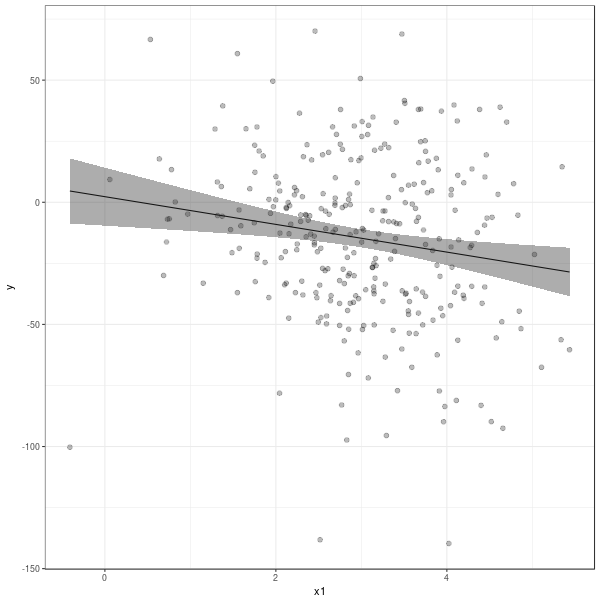
\includegraphics[width=.9\linewidth]{fig-fitted-value-1.png}
\end{center}

There are many options avaiable with the \texttt{gge\_fit()} function. We can at once:
\begin{itemize}
\item Compare fitted values for different groups
\item Compare fitted values for different model specifications, given a list of models
\item Create a grid of plots with fitted values for different groups and model specifications
\end{itemize}

\begin{enumerate}
\item Fitted values for different groups
\label{sec:orgf737267}


\lstset{numbers=left,language=r,label= ,caption= ,captionpos=b}
\begin{lstlisting}
model.g3 %>% gge_fit(., data, 'y', "x2", cat.values=list(cat2=c('a',"b")))
\end{lstlisting}

\begin{center}
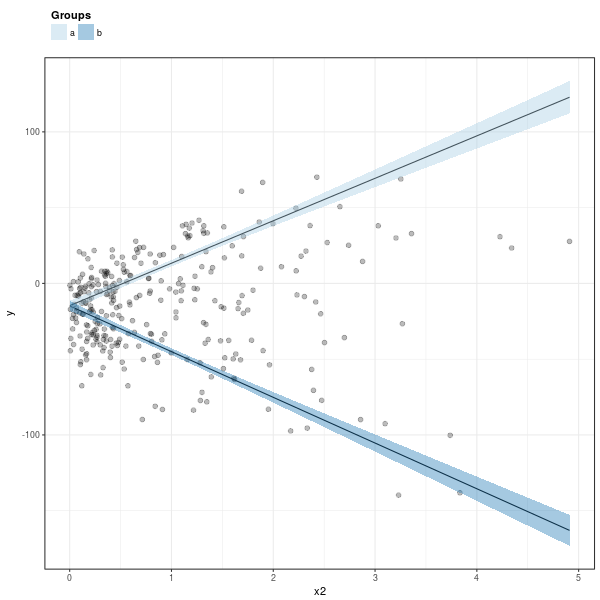
\includegraphics[width=.9\linewidth]{fig-fiited-cat-1.png}
\end{center}

\lstset{numbers=left,language=r,label= ,caption= ,captionpos=b}
\begin{lstlisting}
g1 = model.g3 %>% gge_fit(., data, 'y', "x2",  cat.values=list(cat2=c('a')), title='Variable cat2 fixed at a')
g2 = model.g3 %>% gge_fit(., data, 'y', "x2",  cat.values=list(cat2=c('b')), title='Variable cat2 fixed at b')
ggpubr::ggarrange(g1,g2)
\end{lstlisting}

\begin{center}
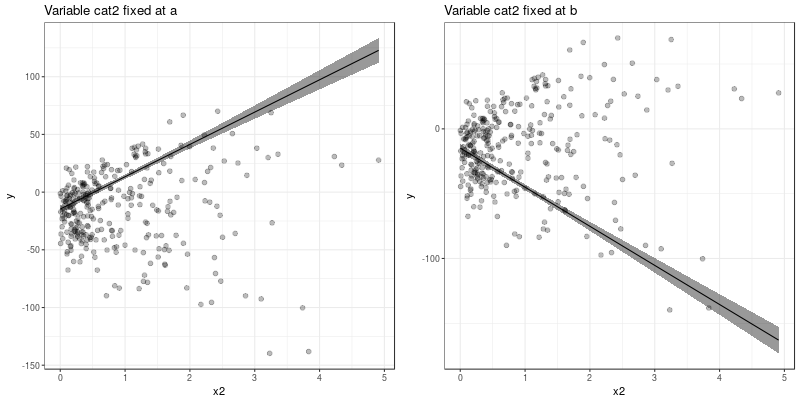
\includegraphics[width=.9\linewidth]{fig-fiited-cat-2.png}
\end{center}


\lstset{numbers=left,language=r,label= ,caption= ,captionpos=b}
\begin{lstlisting}
model.g3 %>% gge_fit(., data, 'y', "x2", facets='cat2' )
\end{lstlisting}

\begin{center}
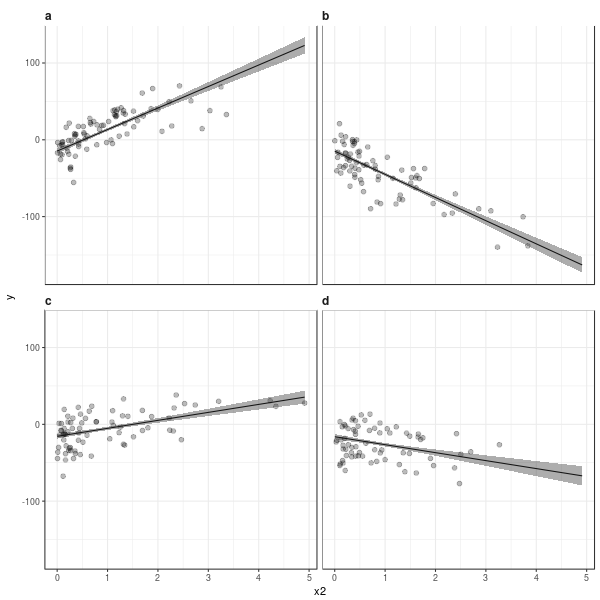
\includegraphics[width=.9\linewidth]{fig-fiited-cat-3.png}
\end{center}

\lstset{numbers=left,language=r,label= ,caption= ,captionpos=b}
\begin{lstlisting}
model.g3 %>% edar::gge_fit(., data, 'y', 'x1', facets='cat2', pch.col.cat='cat1', pch.col.palette=c(brewer="Set2"))
\end{lstlisting}

\begin{center}
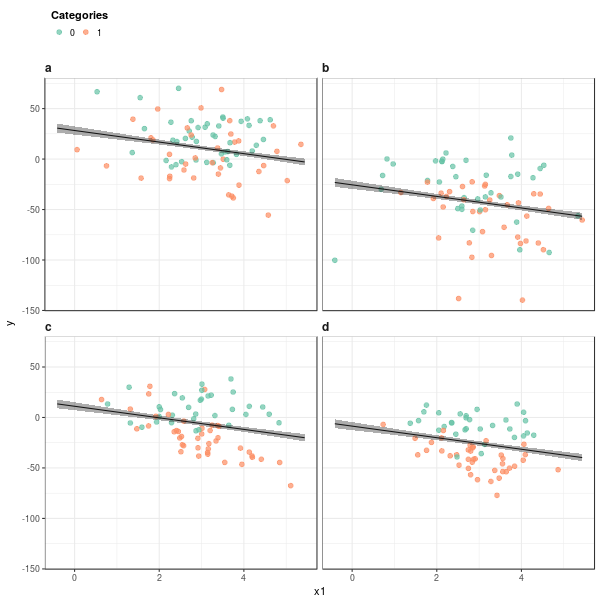
\includegraphics[width=.9\linewidth]{fig-fitted-4.png}
\end{center}

We can also compare a list of models

\lstset{numbers=left,language=r,label= ,caption= ,captionpos=b}
\begin{lstlisting}
formulas = list("Model 1" = formula1, "Model 2" = formula2, "Model 3" = formula3)
models   = list("Model 1" = model.g1, "Model 2" = model.g2, "Model 3" = model.g3)

models %>%  gge_fit(., data, "y", "x2", formulas)

\end{lstlisting}

\begin{center}
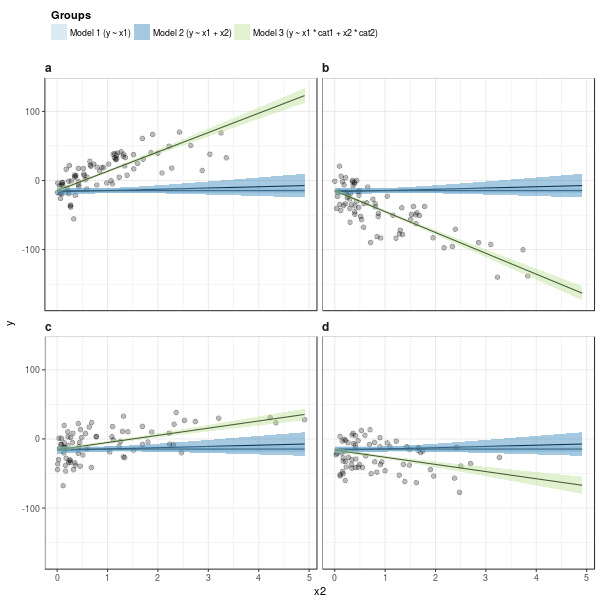
\includegraphics[width=.9\linewidth]{fig-fitted-many-models-1.png}
\end{center}



\lstset{numbers=left,language=r,label= ,caption= ,captionpos=b}
\begin{lstlisting}
formulas = list("Model 1" = formula1, "Model 2" = formula2, "Model 3" = formula3)
models   = list("Model 1" = model.g1, "Model 2" = model.g2, "Model 3" = model.g3)

models %>%  gge_fit(., data, "y", "x2", formulas,  legend.ncol.fill=3, facets='cat2')

\end{lstlisting}

\begin{center}
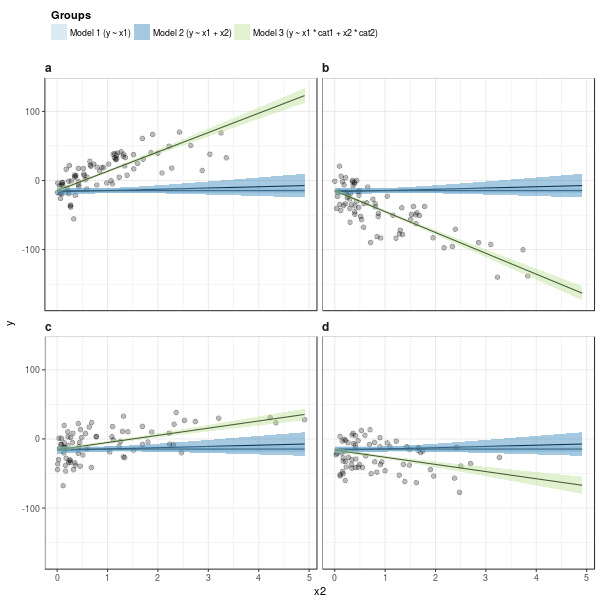
\includegraphics[width=.9\linewidth]{fig-fitted-many-models-1.png}
\end{center}


The same applies for logistic regressions.


\lstset{numbers=left,language=r,label= ,caption= ,captionpos=b}
\begin{lstlisting}
formula.bin1 = y.bin ~ x1+x2
formula.bin2 = y.bin ~ x1+x2*cat2
model.bin1   = glm(formula.bin1, data=data, family='binomial')
model.bin2   = glm(formula.bin2, data=data, family='binomial')

formulas = list("Model 1" = formula.bin1, "Model 2" = formula.bin2)
models   = list("Model 1" = model.bin1, "Model 2" = model.bin2)

models %>%  gge_fit(., data, "y.bin", "x1", formulas)


\end{lstlisting}

\begin{center}
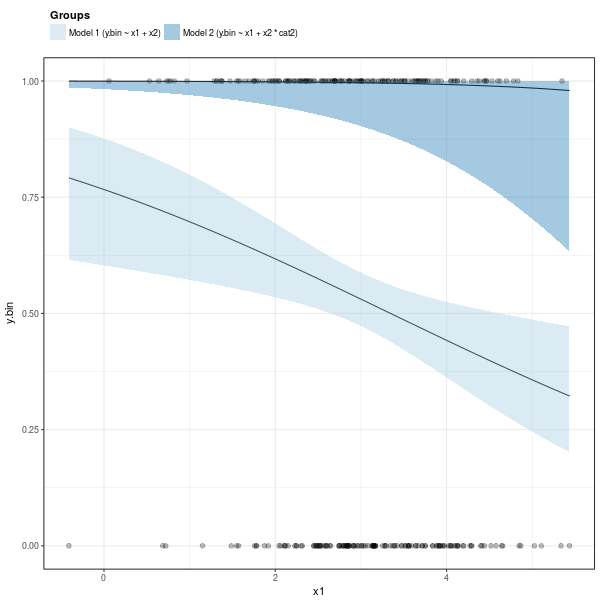
\includegraphics[width=.9\linewidth]{fig-fitted-many-models-bin.png}
\end{center}

\lstset{numbers=left,language=r,label= ,caption= ,captionpos=b}
\begin{lstlisting}
formula.bin1 = y.bin ~ x1+x2
formula.bin2 = y.bin ~ x1+x2*cat2
model.bin1   = glm(formula.bin1, data=data, family='binomial')
model.bin2   = glm(formula.bin2, data=data, family='binomial')

formulas = list("Model 1" = formula.bin1, "Model 2" = formula.bin2)
models   = list("Model 1" = model.bin1, "Model 2" = model.bin2)
models %>%  gge_fit(., data, "y.bin", "x2", formulas, facets='cat2')

\end{lstlisting}

\begin{center}
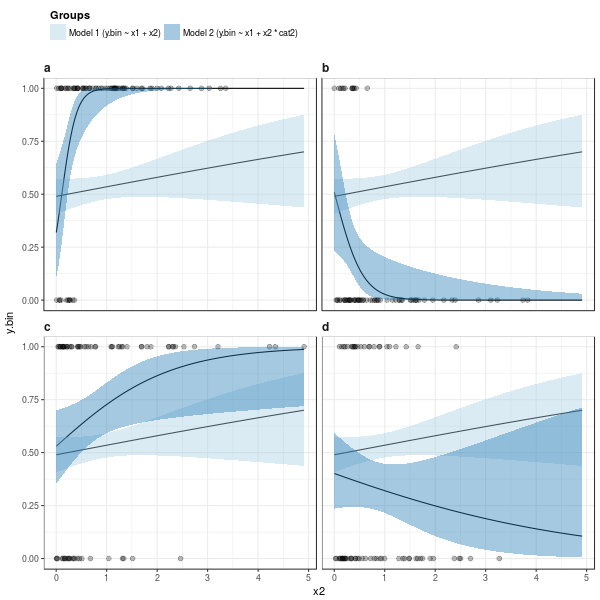
\includegraphics[width=.9\linewidth]{fig-fitted-many-models-bin-2.png}
\end{center}
\end{enumerate}

\subsubsection{Plot with coefficients (dotwisker)}
\label{sec:org343e683}
The \texttt{edar} package also provides a wrap function for the \texttt{dotwisker()} plot from the package with same name. As before, the function accepts list of models or tidy summaries of the estimation. There are also options to use robust standard errors in the plot.

\lstset{numbers=left,language=r,label= ,caption= ,captionpos=b}
\begin{lstlisting}
models=tidye(list('Standard Model'=model.bin2)) %>%
    dplyr::bind_rows(tidye(list('Robust std. error'=model.bin2), hc=T) )
gge_coef(models, model.id='model')
\end{lstlisting}

\begin{center}
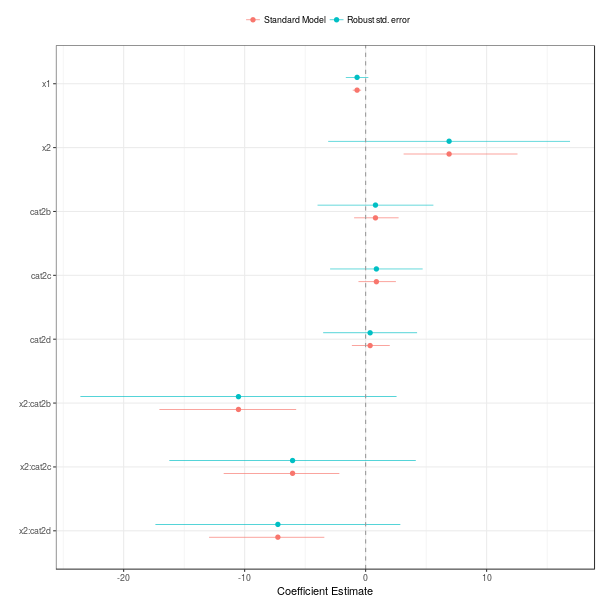
\includegraphics[width=.9\linewidth]{dotwisker-1.png}
\end{center}
\subsection{Multiple-imputation and post-stratification}
\label{sec:org3544888}
Multiple imputation and post-stratification are easy to conduct. The options are limited. Tha package \texttt{survey} and the package \texttt{mice} contain more options.

Here is an example of multiple imputation for two models with different output variables.

\lstset{numbers=left,language=r,label= ,caption= ,captionpos=b}
\begin{lstlisting}
data = tibble::data_frame(x1 = rnorm(200,3,1),
                          x2 = rexp(200),
                          cat.var  = sample(c(0,1), 200, replace=T),
                          cat.var2 = sample(letters[1:4], 200, replace=T),
                          y1 = 10*x1*cat.var+rnorm(200,0,10) +
                              3*x2*(6*(cat.var2=='a') -3*(cat.var2=='b') +
                                    1*(cat.var2=='c') +1*(cat.var2=='d')),
                          y2 = -10*x1*cat.var+rnorm(200,0,10) +
                              10*x2*(3*(cat.var2=='a') -3*(cat.var2=='b') +
                                     1*(cat.var2=='c') -1*(cat.var2=='d'))
                          )  %>%
    dplyr::mutate(cat.var=as.factor(cat.var)) 
data$x1[sample(1:nrow(data), 10)] = NA


formula = "x1*cat.var+x2*cat.var2"
imp = emultimputation(data, formula,  dep.vars = c("y1", "y2"), ind.vars=c("x1", "x2", "cat.var", "cat.var2"))
imp$y1 %>%
    kableExtra::kable(., "latex", booktabs = T ) %>%
    kableExtra::kable_styling(latex_options = c("scale_down"))

\end{lstlisting}

\begin{table}[H]
\centering
\resizebox{\linewidth}{!}{
\begin{tabular}{lrrrrrrrrrr}
\toprule
term & estimate & se & t & df & p.value & low.95 & high.95 & nmis & fmi & lambda\\
\midrule
(Intercept) & 1.2196 & 3.4872 & 0.3497 & 183.9 & 0.7269 & -5.660 & 8.100 &  & 0.0218 & 0.0112\\
x1 & 0.3293 & 0.8412 & 0.3914 & 182.8 & 0.6959 & -1.331 & 1.989 & 10 & 0.0245 & 0.0139\\
cat.var2 & -4.9541 & 4.5860 & -1.0802 & 158.3 & 0.2817 & -14.012 & 4.104 & 0 & 0.0638 & 0.0521\\
x2 & 17.2509 & 1.3802 & 12.4993 & 181.6 & 0.0000 & 14.528 & 19.974 & 0 & 0.0274 & 0.0167\\
cat.var2b & 0.5389 & 3.0200 & 0.1784 & 176.4 & 0.8586 & -5.421 & 6.499 &  & 0.0375 & 0.0266\\
\addlinespace
cat.var2c & -3.7201 & 3.0468 & -1.2210 & 179.1 & 0.2237 & -9.732 & 2.292 &  & 0.0325 & 0.0218\\
cat.var2d & -2.1013 & 3.0617 & -0.6863 & 177.7 & 0.4934 & -8.143 & 3.941 &  & 0.0351 & 0.0243\\
x1:cat.var2 & 10.5961 & 1.4690 & 7.2130 & 155.1 & 0.0000 & 7.694 & 13.498 &  & 0.0680 & 0.0560\\
x2:cat.var2b & -26.7177 & 2.0414 & -13.0880 & 185.4 & 0.0000 & -30.745 & -22.690 &  & 0.0173 & 0.0068\\
x2:cat.var2c & -12.7266 & 1.8036 & -7.0563 & 181.8 & 0.0000 & -16.285 & -9.168 &  & 0.0270 & 0.0163\\
x2:cat.var2d & -13.2621 & 2.0852 & -6.3601 & 184.5 & 0.0000 & -17.376 & -9.148 &  & 0.0201 & 0.0095\\
\bottomrule
\end{tabular}}
\end{table}


\lstset{numbers=left,language=r,label= ,caption= ,captionpos=b}
\begin{lstlisting}
imp$y2 %>%
    kableExtra::kable(., "latex", booktabs = T ) %>%
    kableExtra::kable_styling(latex_options = c("scale_down"))

\end{lstlisting}

\begin{table}[H]
\centering
\resizebox{\linewidth}{!}{
\begin{tabular}{lrrrrrrrrrr}
\toprule
term & estimate & se & t & df & p.value & low.95 & high.95 & nmis & fmi & lambda\\
\midrule
(Intercept) & 7.0397 & 3.4878 & 2.0184 & 122.8 & 0.0457 & 0.1357 & 13.9437 &  & 0.1089 & 0.0946\\
x1 & -0.4107 & 0.8368 & -0.4908 & 127.6 & 0.6244 & -2.0664 & 1.2450 & 10 & 0.1028 & 0.0888\\
cat.var2 & 2.9983 & 4.5419 & 0.6601 & 104.7 & 0.5106 & -6.0077 & 12.0043 & 0 & 0.1344 & 0.1181\\
x2 & 27.6086 & 1.3153 & 20.9904 & 185.2 & 0.0000 & 25.0137 & 30.2035 & 0 & 0.0178 & 0.0072\\
cat.var2b & -5.6630 & 2.9412 & -1.9254 & 152.0 & 0.0560 & -11.4740 & 0.1479 &  & 0.0719 & 0.0598\\
\addlinespace
cat.var2c & -6.4962 & 3.0161 & -2.1538 & 129.7 & 0.0331 & -12.4634 & -0.5290 &  & 0.1000 & 0.0862\\
cat.var2d & -2.4124 & 3.0181 & -0.7993 & 134.9 & 0.4255 & -8.3812 & 3.5564 &  & 0.0933 & 0.0800\\
x1:cat.var2 & -10.6894 & 1.4361 & -7.4433 & 111.9 & 0.0000 & -13.5349 & -7.8439 &  & 0.1240 & 0.1085\\
x2:cat.var2b & -58.4786 & 1.9527 & -29.9479 & 186.0 & 0.0000 & -62.3309 & -54.6264 &  & 0.0150 & 0.0045\\
x2:cat.var2c & -17.1821 & 1.7227 & -9.9738 & 182.8 & 0.0000 & -20.5811 & -13.7832 &  & 0.0245 & 0.0139\\
x2:cat.var2d & -39.4869 & 1.9911 & -19.8313 & 186.8 & 0.0000 & -43.4149 & -35.5589 &  & 0.0118 & 0.0012\\
\bottomrule
\end{tabular}}
\end{table}


Post-stratification for simple probabilistic sample is also straightforward.

\lstset{numbers=left,language=r,label= ,caption= ,captionpos=b}
\begin{lstlisting}
data = tibble::data_frame(educ = sample(c("Low", "High"), 200, T), gender=sample(c('Man', "Woman"), 200, T), other.variable=rnorm(200)) 
pop.prop = tibble::data_frame(educ = c("Low", "High"))  %>%
    tidyr::crossing(gender=c("Man", "Woman")) %>%
    dplyr::mutate(Freq = 100*c(.3,.25,.3,.15)) 

epoststrat(data, pop.prop, strata = ~educ+gender) 
\end{lstlisting}

\begin{verbatim}
$weights
  [1] 0.5455 0.2542 0.7895 0.2542 0.5455 0.7895 0.5208 0.7895 0.2542
 [10] 0.2542 0.5208 0.5455 0.7895 0.5455 0.5455 0.2542 0.5208 0.7895
 [19] 0.5455 0.5455 0.5208 0.5455 0.5208 0.2542 0.5208 0.2542 0.7895
 [28] 0.7895 0.5455 0.7895 0.5208 0.5455 0.2542 0.7895 0.2542 0.5208
 [37] 0.7895 0.2542 0.7895 0.5208 0.2542 0.2542 0.5455 0.5208 0.5455
 [46] 0.5208 0.5455 0.5455 0.7895 0.5208 0.7895 0.2542 0.5455 0.2542
 [55] 0.5455 0.7895 0.5208 0.7895 0.2542 0.2542 0.5455 0.2542 0.5455
 [64] 0.2542 0.5455 0.2542 0.2542 0.5208 0.2542 0.2542 0.2542 0.5455
 [73] 0.5208 0.2542 0.5208 0.5455 0.2542 0.5455 0.2542 0.5455 0.5455
 [82] 0.7895 0.7895 0.2542 0.2542 0.7895 0.2542 0.7895 0.5208 0.5455
 [91] 0.5208 0.7895 0.5208 0.5455 0.5208 0.7895 0.5455 0.2542 0.5455
[100] 0.7895 0.5208 0.5208 0.2542 0.5208 0.2542 0.2542 0.7895 0.5208
[109] 0.2542 0.7895 0.5455 0.7895 0.5455 0.5455 0.5455 0.2542 0.2542
[118] 0.7895 0.5208 0.2542 0.5455 0.2542 0.2542 0.5208 0.2542 0.5208
[127] 0.7895 0.2542 0.5455 0.7895 0.5455 0.5455 0.2542 0.5455 0.5455
[136] 0.2542 0.5455 0.2542 0.2542 0.5208 0.5455 0.2542 0.5208 0.2542
[145] 0.5455 0.5455 0.5208 0.7895 0.2542 0.2542 0.5208 0.5455 0.5208
[154] 0.5208 0.5455 0.5208 0.7895 0.7895 0.5208 0.5455 0.5208 0.7895
[163] 0.7895 0.7895 0.5455 0.7895 0.5208 0.5455 0.5208 0.2542 0.2542
[172] 0.2542 0.5455 0.5208 0.2542 0.5455 0.5208 0.2542 0.5208 0.5208
[181] 0.5455 0.5208 0.5455 0.5208 0.7895 0.5208 0.2542 0.5455 0.5208
[190] 0.2542 0.2542 0.5208 0.5455 0.5455 0.2542 0.5208 0.5455 0.2542
[199] 0.7895 0.7895

$weights.trimmed
  [1] 0.5455 0.2542 0.7895 0.2542 0.5455 0.7895 0.5208 0.7895 0.2542
 [10] 0.2542 0.5208 0.5455 0.7895 0.5455 0.5455 0.2542 0.5208 0.7895
 [19] 0.5455 0.5455 0.5208 0.5455 0.5208 0.2542 0.5208 0.2542 0.7895
 [28] 0.7895 0.5455 0.7895 0.5208 0.5455 0.2542 0.7895 0.2542 0.5208
 [37] 0.7895 0.2542 0.7895 0.5208 0.2542 0.2542 0.5455 0.5208 0.5455
 [46] 0.5208 0.5455 0.5455 0.7895 0.5208 0.7895 0.2542 0.5455 0.2542
 [55] 0.5455 0.7895 0.5208 0.7895 0.2542 0.2542 0.5455 0.2542 0.5455
 [64] 0.2542 0.5455 0.2542 0.2542 0.5208 0.2542 0.2542 0.2542 0.5455
 [73] 0.5208 0.2542 0.5208 0.5455 0.2542 0.5455 0.2542 0.5455 0.5455
 [82] 0.7895 0.7895 0.2542 0.2542 0.7895 0.2542 0.7895 0.5208 0.5455
 [91] 0.5208 0.7895 0.5208 0.5455 0.5208 0.7895 0.5455 0.2542 0.5455
[100] 0.7895 0.5208 0.5208 0.2542 0.5208 0.2542 0.2542 0.7895 0.5208
[109] 0.2542 0.7895 0.5455 0.7895 0.5455 0.5455 0.5455 0.2542 0.2542
[118] 0.7895 0.5208 0.2542 0.5455 0.2542 0.2542 0.5208 0.2542 0.5208
[127] 0.7895 0.2542 0.5455 0.7895 0.5455 0.5455 0.2542 0.5455 0.5455
[136] 0.2542 0.5455 0.2542 0.2542 0.5208 0.5455 0.2542 0.5208 0.2542
[145] 0.5455 0.5455 0.5208 0.7895 0.2542 0.2542 0.5208 0.5455 0.5208
[154] 0.5208 0.5455 0.5208 0.7895 0.7895 0.5208 0.5455 0.5208 0.7895
[163] 0.7895 0.7895 0.5455 0.7895 0.5208 0.5455 0.5208 0.2542 0.2542
[172] 0.2542 0.5455 0.5208 0.2542 0.5455 0.5208 0.2542 0.5208 0.5208
[181] 0.5455 0.5208 0.5455 0.5208 0.7895 0.5208 0.2542 0.5455 0.5208
[190] 0.2542 0.2542 0.5208 0.5455 0.5455 0.2542 0.5208 0.5455 0.2542
[199] 0.7895 0.7895
\end{verbatim}




\bibliographystyle{apalike}
\bibliography{../../../../../../../../references/references}
\end{document}
